% This is samplepaper.tex, a sample chapter demonstrating the
% LLNCS macro package for Springer Computer Science proceedings;
% Version 2.20 of 2017/10/04
%
\documentclass[runningheads]{llncs}

\usepackage{graphicx}   % Images

\usepackage{setspace}   % Spacing

% If you use the hyperref package, please uncomment the following line
% to display URLs in blue roman font according to Springer's eBook style:
% \renewcommand\UrlFont{\color{blue}\rmfamily}

\begin{document}
% Title
\title{Solver of Tricky Triple Puzzles Based on Constraint Programming}
% Abbreviated Title
\titlerunning{Tricky Triple Solver}

% Authors
\author{Ângelo Daniel Pereira Mendes Moura\orcidID{upXXXXXXXX@fe.up.pt} \\
\and Clara Alves Martins\orcidID{up201806528@fe.up.pt}}
\authorrunning{Ângelo Moura \and Clara Martins}

% Institutes
\institute{Faculty of Engineering of the University of Porto \\
\url{https://www.fe.up.pt}}

% Date for the report
\date{\today}

\maketitle              % typeset the header of the contribution

\begin{abstract}
In this article, we show how to use constraint programming to solve Tricky Triple Puzzles.
We present a consistent method to analyze these puzzles and to obtain a solution to them.

\keywords{tricky-triple \and prolog \and clpfd \and constraint-programming.}
\end{abstract}

\newpage

% Table of Contents
\setcounter{tocdepth}{2} % Show sections + subsections
\doublespacing % Spacing
\tableofcontents
\singlespacing

\newpage

% Contents
\section{Introduction}
This project consists of building a program, in Logic Programming with Restrictions,
    for solving a combinatorial decision.
The problems studied are Tricky Triple Puzzles, which are grid puzzles. 
To do so, we will analyze these problems and proceed to implement our solver using SICStus Prolog.
Afterward, we will be discussing the performance results obtained.

\section{Problem Description}
The Tricky Triple puzzles are a type of grid puzzle.
The goal of the puzzle is to fill each of the grid’s white cells with one of 3 symbols,
a square, a circle, or a triangle.
The only rule is that each group of 3 adjacent white cells
    (horizontally, vertically, or diagonally) must contain exactly 2 of one of the symbols.
So, each group of 3 white cells will have 2 of 3 symbols.
Each puzzle below has a unique solution.

\begin{figure}
    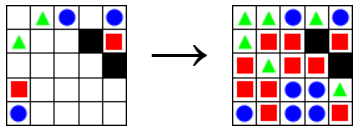
\includegraphics[width=\textwidth]{img/tricky-triple.png}
    \caption{Example of Tricky Triple Puzzles, before and after solving it.} \label{fig1}
\end{figure}

\section{Approach}
\subsection{Decision Variables}
\subsection{Constraints}

\section{Solution Presentation}

\section{Experiments and Results}
\subsection{Dimensional Analysis}
\subsection{Search Strategies}

\section{Conclusions and Future Work}

\section{Section Sample}
\subsection{A Subsection Sample}
Please note that the first paragraph of a section or subsection is
not indented. The first paragraph that follows a table, figure,
equation etc. does not need an indent, either.

Subsequent paragraphs, however, are indented.

\subsubsection{Sample Heading (Third Level)} Only two levels of
headings should be numbered. Lower level headings remain unnumbered;
they are formatted as run-in headings.

\paragraph{Sample Heading (Fourth Level)}
The contribution should contain no more than four levels of
headings. Table~\ref{tab1} gives a summary of all heading levels.

\begin{table}
\caption{Table captions should be placed above the
tables.}\label{tab1}
\begin{tabular}{|l|l|l|}
\hline
Heading level &  Example & Font size and style\\
\hline
Title (centered) &  {\Large\bfseries Lecture Notes} & 14 point, bold\\
1st-level heading &  {\large\bfseries 1 Introduction} & 12 point, bold\\
2nd-level heading & {\bfseries 2.1 Printing Area} & 10 point, bold\\
3rd-level heading & {\bfseries Run-in Heading in Bold.} Text follows & 10 point, bold\\
4th-level heading & {\itshape Lowest Level Heading.} Text follows & 10 point, italic\\
\hline
\end{tabular}
\end{table}


\noindent Displayed equations are centered and set on a separate
line.
\begin{equation}
x + y = z
\end{equation}
Please try to avoid rasterized images for line-art diagrams and
schemas. Whenever possible, use vector graphics instead (see
Fig.~\ref{fig1}).

\begin{figure}

\includegraphics[width=\textwidth]{img/FEUPlogo.png}
\caption{A figure caption is always placed below the illustration.
Please note that short captions are centered, while long ones are
justified by the macro package automatically.} \label{fig1}
\end{figure}

\begin{theorem}
This is a sample theorem. The run-in heading is set in bold, while
the following text appears in italics. Definitions, lemmas,
propositions, and corollaries are styled the same way.
\end{theorem}
%
% the environments 'definition', 'lemma', 'proposition', 'corollary',
% 'remark', and 'example' are defined in the LLNCS documentclass as well.
%
\begin{proof}
Proofs, examples, and remarks have the initial word in italics,
while the following text appears in normal font.
\end{proof}
For citations of references, we prefer the use of square brackets
and consecutive numbers. Citations using labels or the author/year
convention are also acceptable. The following bibliography provides
a sample reference list with entries for journal
% TODO
%articles~\cite{ref_article1}, an LNCS chapter~\cite{ref_lncs1}, a
%book~\cite{ref_book1}, proceedings without editors~\cite{ref_proc1},
%and a homepage~\cite{ref_url1}. Multiple citations are grouped
%\cite{ref_article1,ref_lncs1,ref_book1},
%\cite{ref_article1,ref_book1,ref_proc1,ref_url1}.
%
% ---- Bibliography ----
%
% BibTeX users should specify bibliography style 'splncs04'.
% References will then be sorted and formatted in the correct style.
%
% \bibliographystyle{splncs04}
% \bibliography{mybibliography}
%
\begin{thebibliography}{8}
\bibitem{ref_article1}
Author, F.: Article title. Journal \textbf{2}(5), 99--110 (2016)

\bibitem{ref_lncs1}
Author, F., Author, S.: Title of a proceedings paper. In: Editor,
F., Editor, S. (eds.) CONFERENCE 2016, LNCS, vol. 9999, pp. 1--13.
Springer, Heidelberg (2016). \doi{10.10007/1234567890}

\bibitem{ref_book1}
Author, F., Author, S., Author, T.: Book title. 2nd edn. Publisher,
Location (1999)

\bibitem{ref_proc1}
Author, A.-B.: Contribution title. In: 9th International Proceedings
on Proceedings, pp. 1--2. Publisher, Location (2010)

\bibitem{ref_url1}
LNCS Homepage, \url{http://www.springer.com/lncs}. Last accessed 4
Oct 2017
\end{thebibliography}

\end{document}
